\documentclass[12pt]{article}
\usepackage{fullpage}
\usepackage[utf8]{inputenc}
\usepackage{graphicx}
\usepackage[english]{babel}
\usepackage{float}
\usepackage{natbib}
\usepackage{authblk}
\usepackage{url}
\usepackage[section]{placeins}
\usepackage{wrapfig, framed}

\title{\textbf{Project 7 Report : Convolutional Neural Networks}}
\author{Sajal Kumar}
\date{}

\begin{document}
\maketitle

\section*{Implementation details on parameters}

My implementation allows change to the following parameters.

\begin{itemize}
\item \texttt{batch\_size} : Size of one batch when training the CNN using mini-batches (Default : 100).
\item \texttt{random\_seed} : Random state/ seed for CNN, batch generation, etc (Default : 1).
\item \texttt{learning\_rate} : Learning rate for CNN optimizer (Default : $1e-4$).
\item \texttt{epochs} : Number of iteration the CNN would go through before convergence (Default : 10).
\item \texttt{c1\_kernel\_size} : Kernel size for 1st conv layer (Default : 3).
\item \texttt{c2\_kernel\_size} : Kernel size for 2nd conv layer (Default : 3).
\item \texttt{c1\_op\_channel} : Number of open channels for 1st conv layer (Default : 4).
\item \texttt{c2\_op\_channel} : Number of open channels for 2nd conv layer (Default : 2).
\item \texttt{p1\_pool\_size} : Pool size for 1st pool layer (Default : 2).
\item \texttt{p2\_pool\_size} : Pool size for 2nd pool layer (Default : 4).
\end{itemize}

This along with other criteria mentioned in the project description (e.g. padding = `valid', strides = (1, 1), etc.) represent the standard setting. All other parameters, not mentioned in the project description were kept at their default values.

\section*{CNN architecture}

\begin{figure}
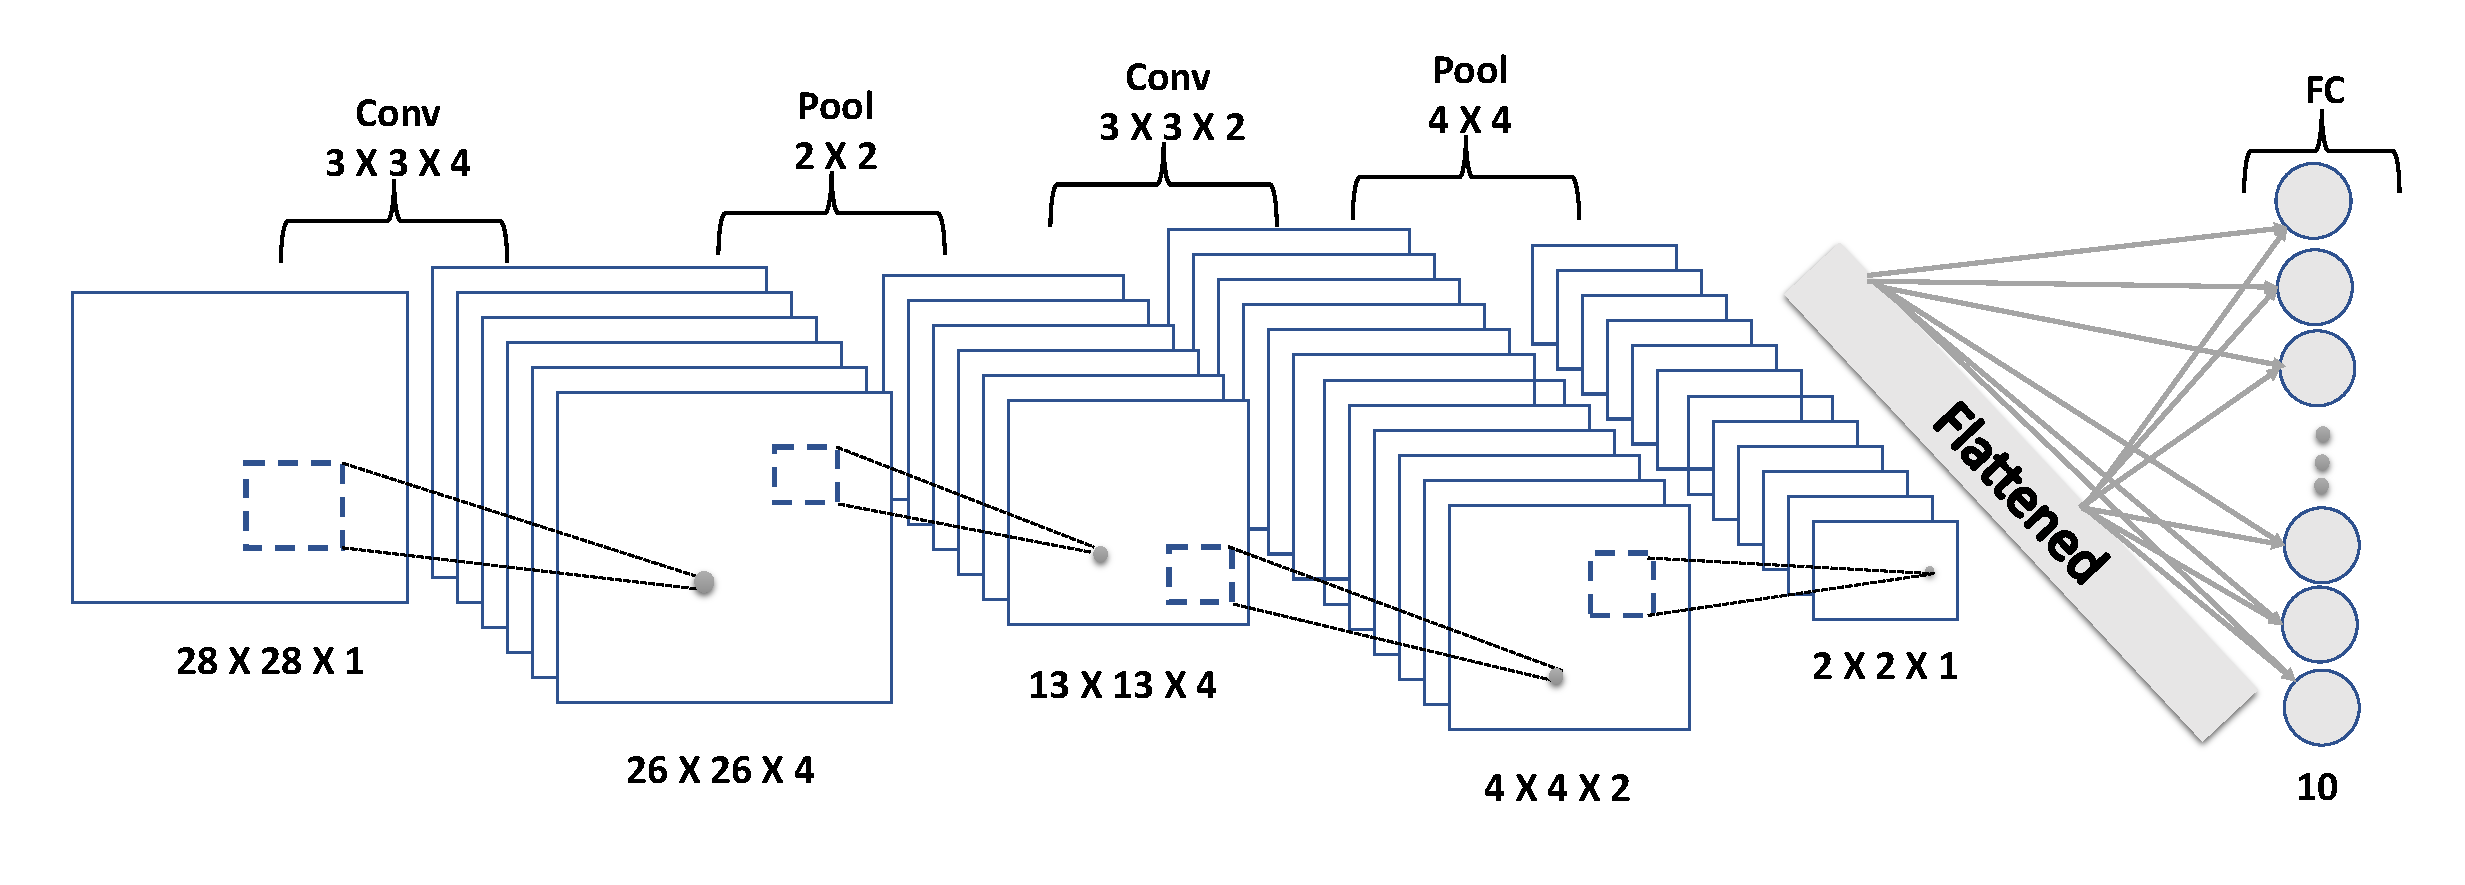
\includegraphics[width=\linewidth]{new_model_cnn_diag.pdf}
\caption{CNN architecture for given configuration.}
\label{fig-1}
\end{figure}

Figure~1 shows the architecture for the configuration provided as a part of the project assignment. The architecture has two convolution tensor layers, two pooling tensor layers and one fully connected tensor layer with 10 output units, that translate to the probability profile of the response. The following are the dimension of each tensor layer.

\begin{itemize}
\item Input layer tensor with dimensions = [\texttt{batch\_size} 28 28 1] 
\item The 1st convolution layer with dimensions = [\texttt{batch\_size} 26 26 4] with kernel size = [3 3] and filters (or number of output channel) = 4.
\item The 1st pooling layer with dimensions = [\texttt{batch\_size} 13 13 4] with pooling size = [2 2].
\item The 2nd convolution layer with dimensions = [\texttt{batch\_size} 4 4 2] with kernel size = [3 3] and filters (or number of output channel) = 2.
\item The 2nd pooling layer with dimensions = [\texttt{batch\_size} 2 2 1] with pooling size = [4 4].
\item The fully connected softmax layer with dimensions = [\texttt{batch\_size} 10], which is also used as the output layer.
\end{itemize}
\section*{Performance evaluation on MNIST}

Here I report predictive accuracy of CNN on MNIST training and testing data. The original data was standardized using the following formula:
\begin{equation}
X_{standard} = \frac{X - \mu}{\sigma_X} 
\end{equation}

Where X is the original feature space of MNIST data set, $\mu$ is a vector of attribute wise mean and $\sigma_X$ is the standard deviation of the entire X feature space.

I also split the data into 3 sets, training, testing and validation. The data was first split (stratified) into 85\% training and 15\% testing. The 85\% training data was then further split into 85\% training data and 15\% validation data.The validation data was used by the CNN to improve upon its performance.

The training data was supplied to the CNN in mini-batches and the loss was computed on the validation data-set. The accuracy obtained on training and testing data was 21.6\% and 21.63\% respectively, which is very poor. To analyze the effect of epochs, I let the CNN run for 200 epochs and while the performance for the 200th epoch was significantly better at 44\% accuracy for both datasets. Figure~2 shows that increasing the epoch number further would not have much effect on the accuracy.

\begin{figure}
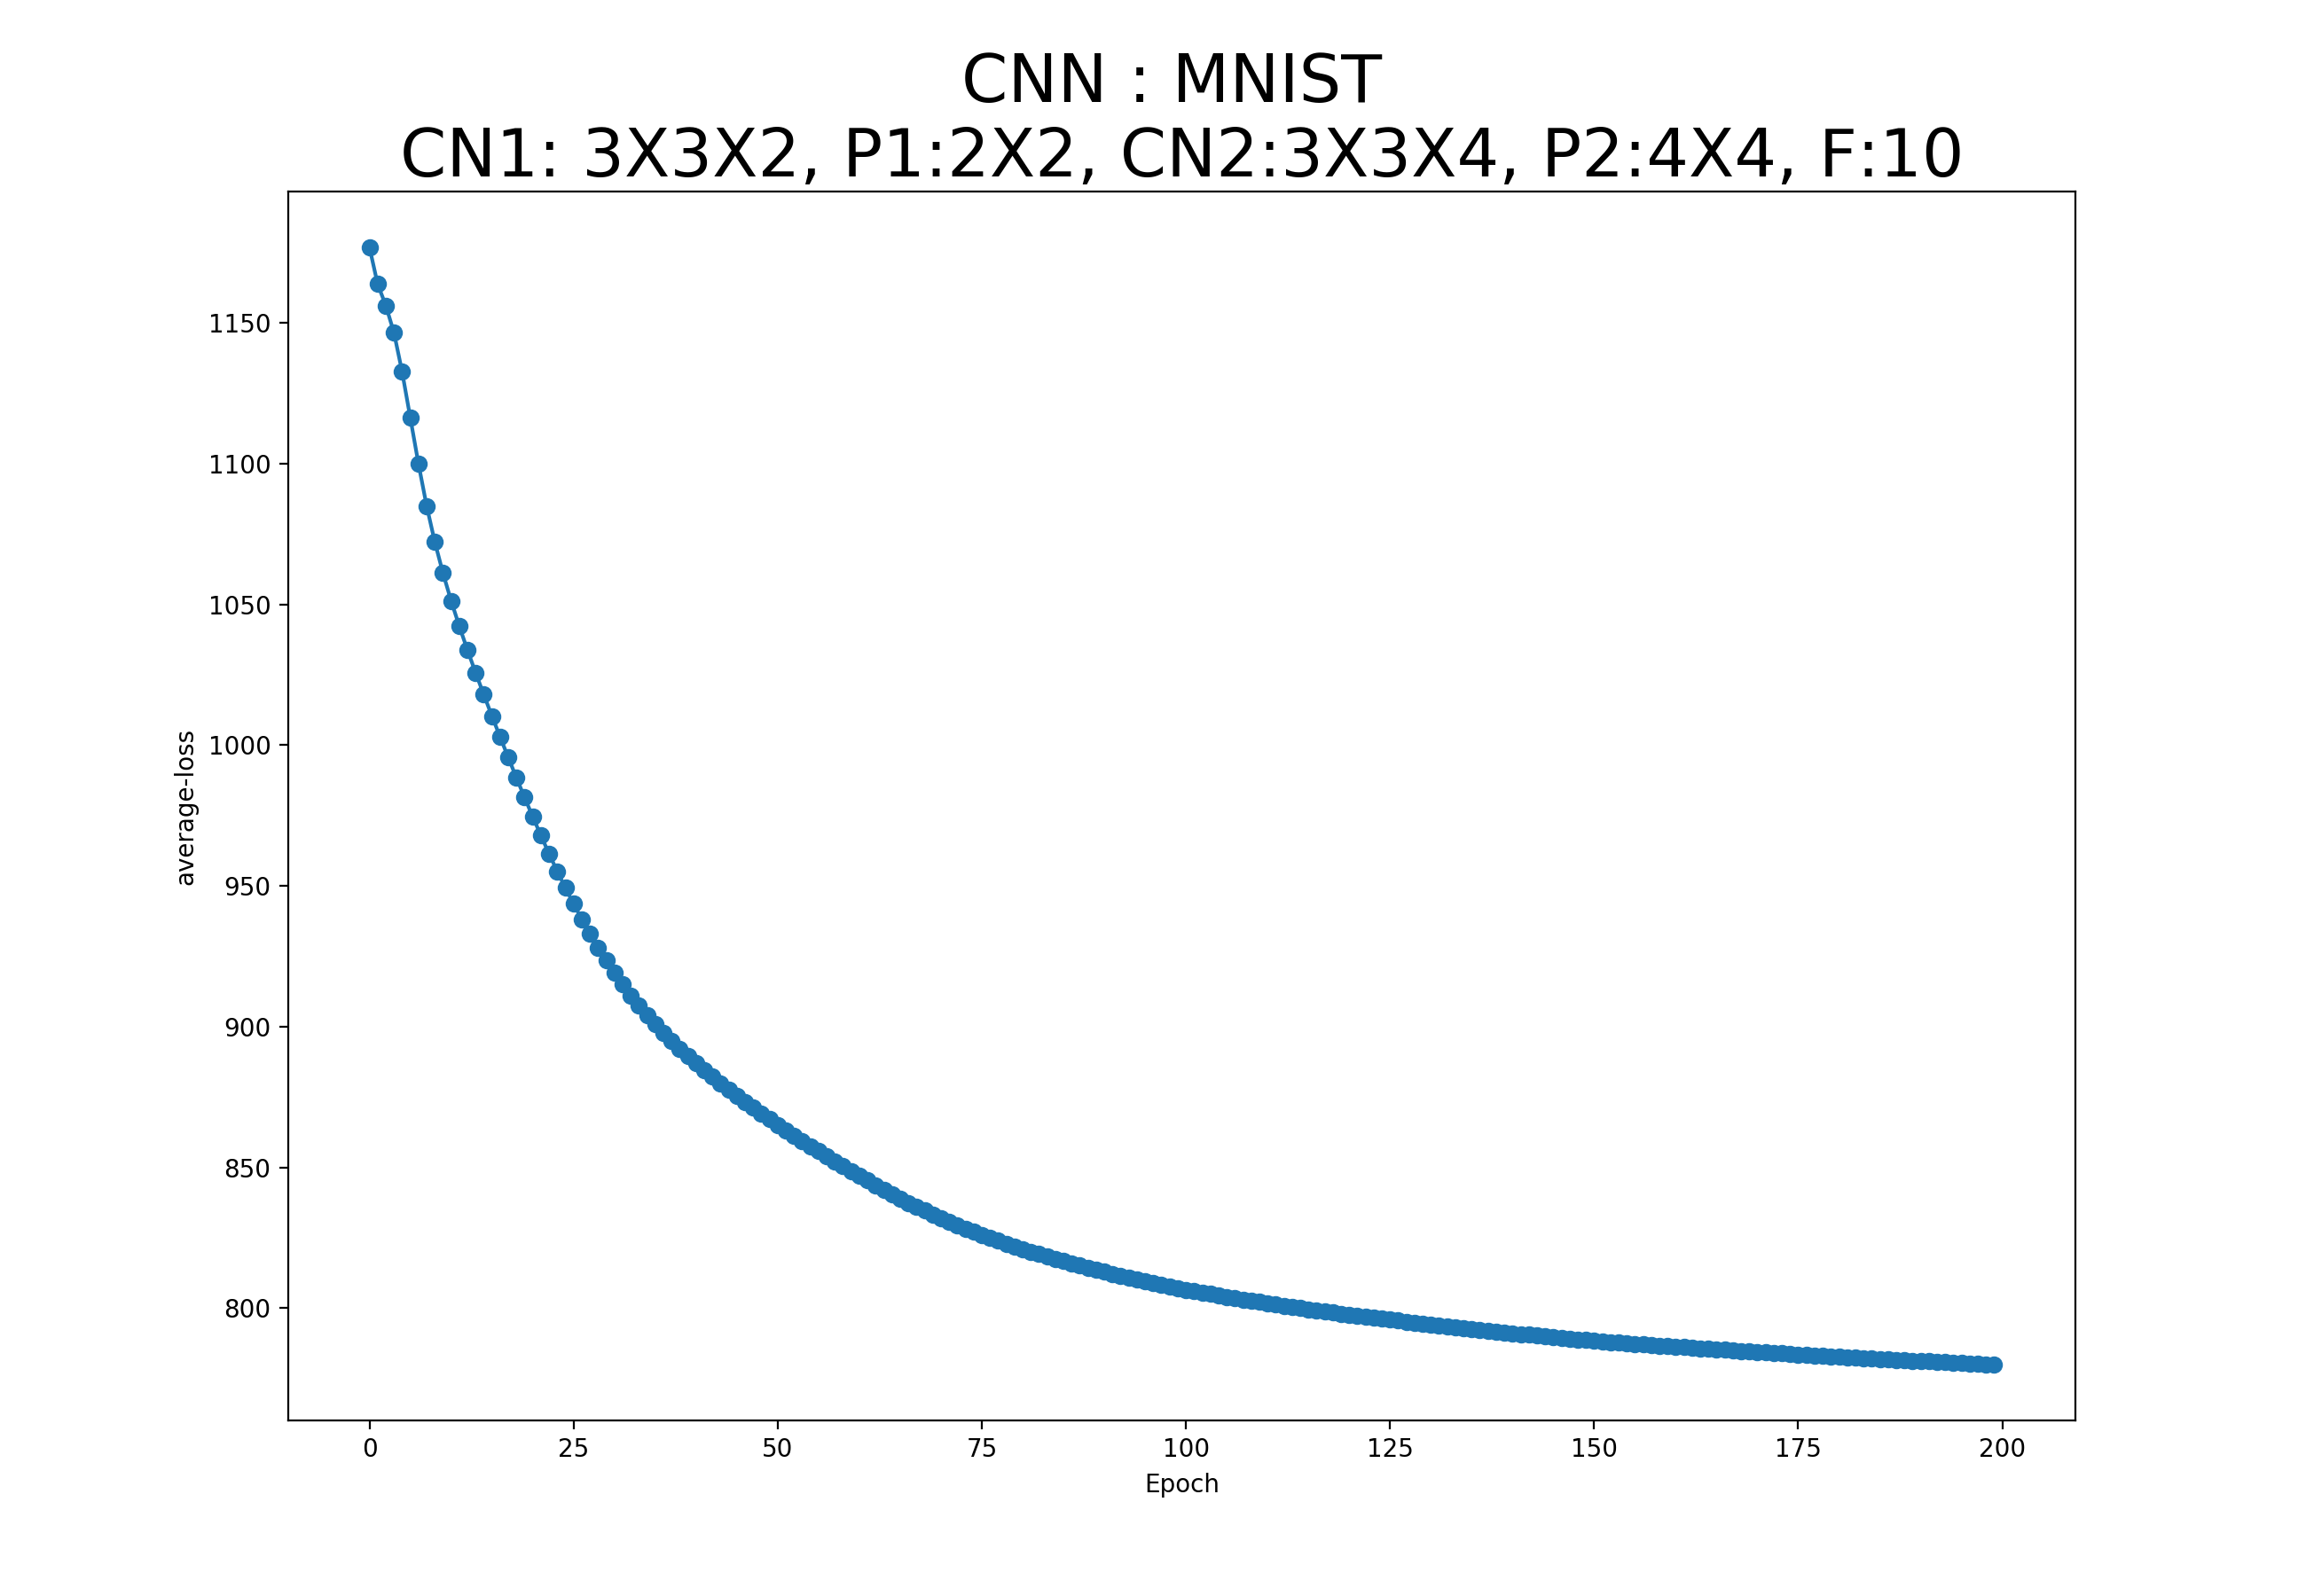
\includegraphics[width=\linewidth]{MNIST-Standard.png}
\caption{Decrease in average loss with epoch on standard setting}
\label{fig-2}
\end{figure}

\section*{A more comprehensive evaluation}

I found that a CNN is quite sensitive to change in its parameters. Here I present 4 configurations touching upon 4 different parameter combinations.

\begin{table}[!hbtp]
\centering
\begin{tabular}{|l|c|c|}
\hline
\textbf{config} & \textbf{pred on train} & \textbf{pred on test} \\\hline
1 & 21.60\% & 21.63\% \\
2 & 97.43\% & 96.45\% \\
3 & 97.45\% & 96.48\% \\
4 & 97.83\% & 97.19\% \\\hline
\end{tabular}
\caption{Performance change for different configuration of parameters.}
\end{table}

Table~1 shows the affect of different parameters on the the CNN, where \textit{config} is given as :

\begin{enumerate}
\item Standard setting
\item \texttt{c1\_kernel\_size}=5, \texttt{c1\_op\_channel}=32, \texttt{c2\_kernel\_size}=5, 

\texttt{c2\_op\_channel}=64 and \texttt{p2\_pool\_size}=2
\item \texttt{c1\_kernel\_size}=5, \texttt{c1\_op\_channel}=32, \texttt{c2\_kernel\_size}=5, 

\texttt{c2\_op\_channel}=64, \texttt{p2\_pool\_size}=2 and \texttt{learning\_rate}=0.01
\item \texttt{batch\_size} = 64, \texttt{c1\_kernel\_size}=5, \texttt{c1\_op\_channel}=32, 

\texttt{c2\_kernel\_size}=5, \texttt{c2\_op\_channel}=64 and \texttt{p2\_pool\_size}=2
\end{enumerate}

As can be seen, there is no contest between config 1 and the others and the reason is that the CNN specific configuration (used in 2) for both convolution / pooling layer works really well for the MNIST dataset. This configuration closely resembles the config used in the textbook with the exception of strides, that are still set at the value that was provided in the project description.

The next interesting effect is of learning rate and batch size, while there is no major change in the final accuracy, figure~3 shows there loss decrease over 10 epochs.

\begin{figure}
\begin{minipage}{\linewidth}
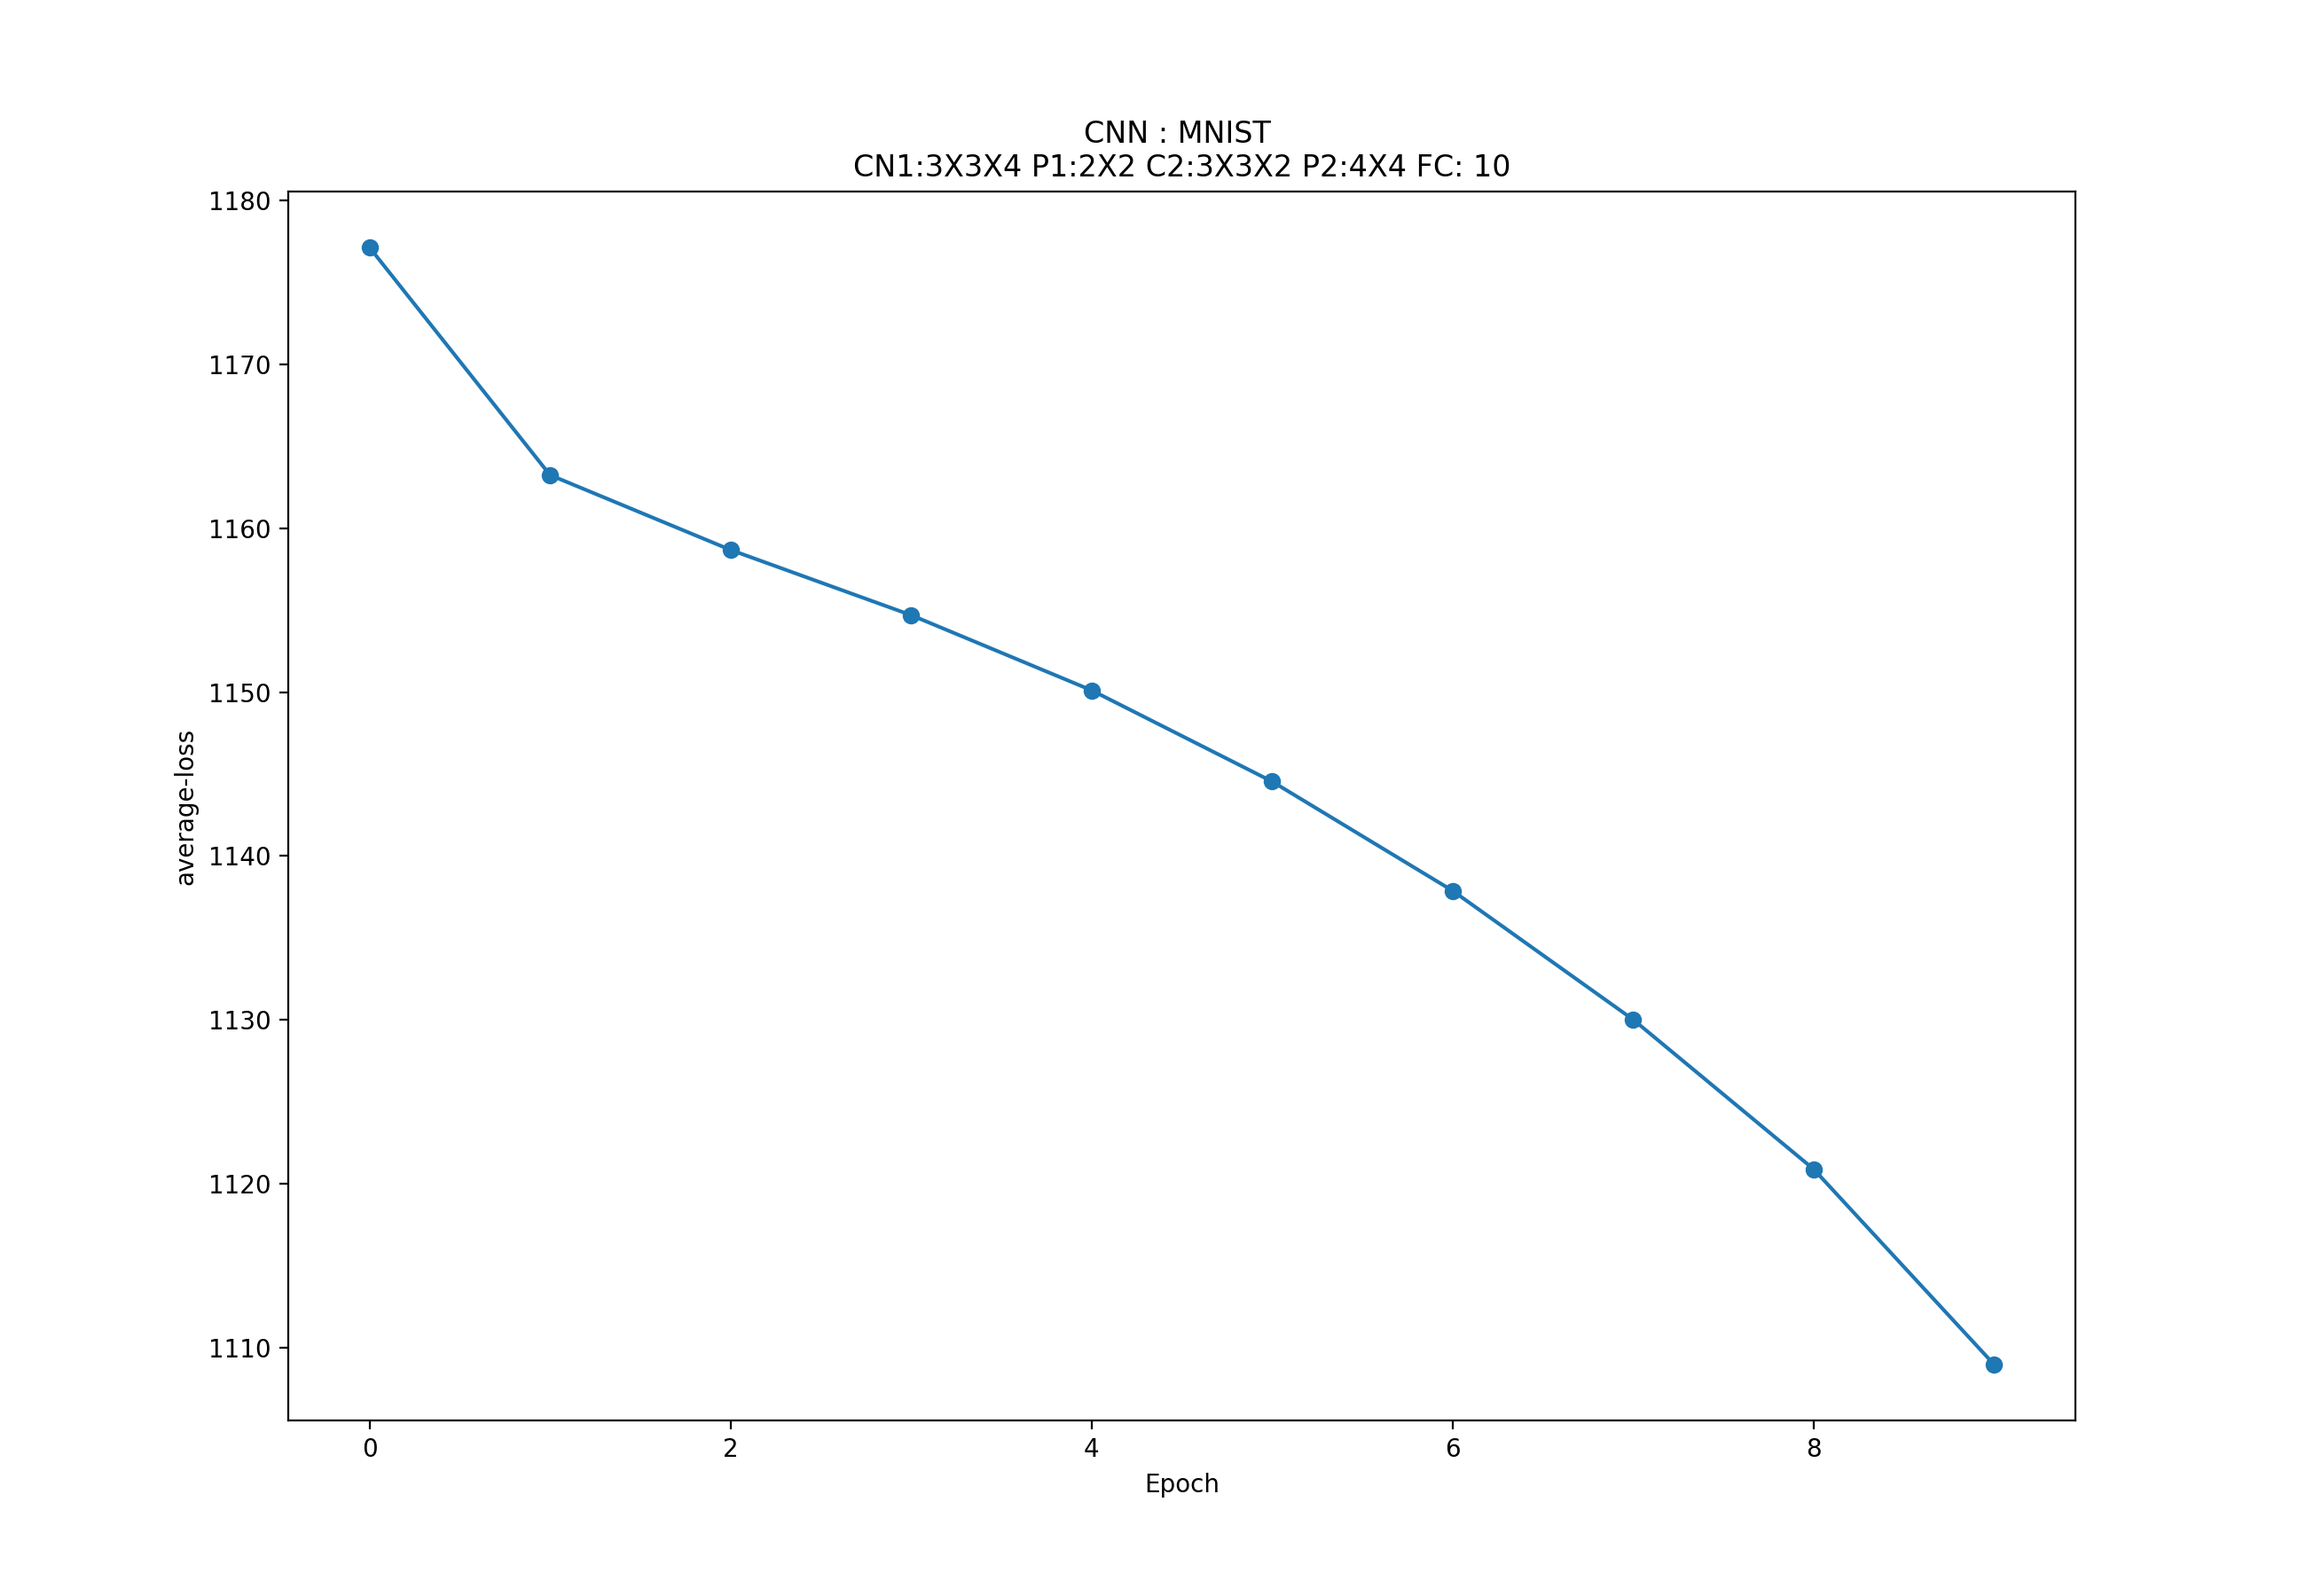
\includegraphics[width=0.5\linewidth]{MNIST-loss-decrease-CNNstandard.png}
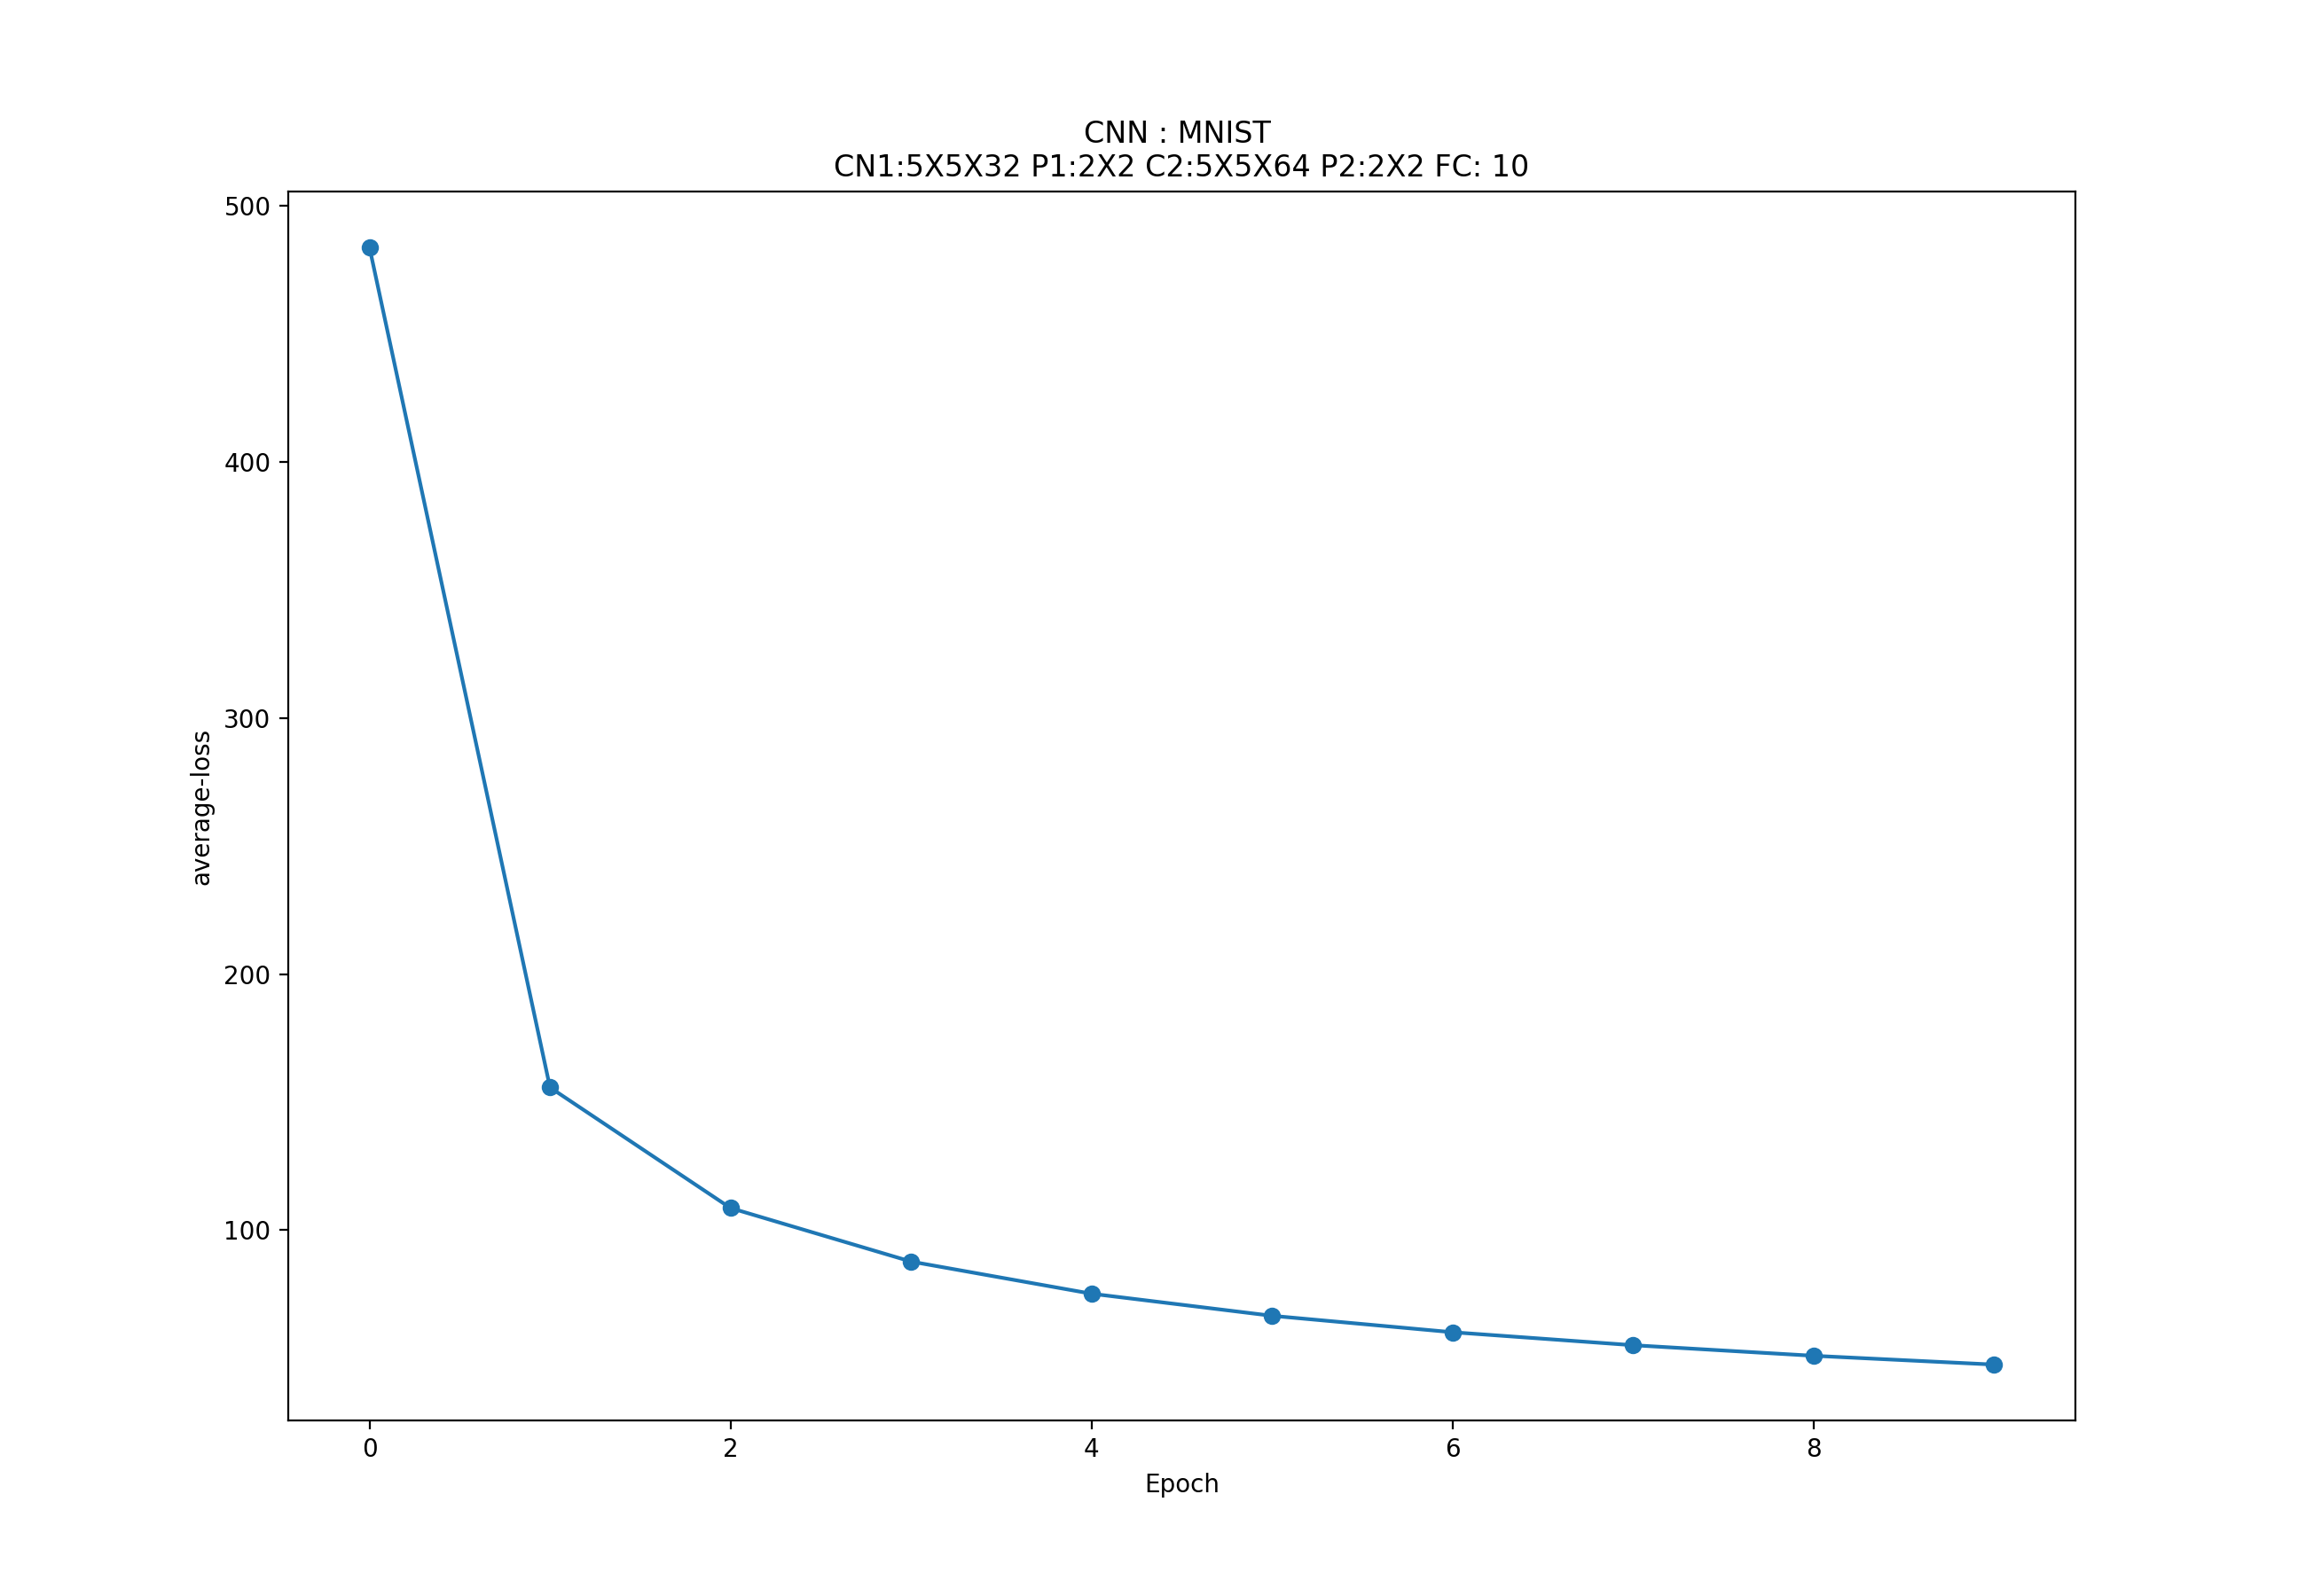
\includegraphics[width=0.5\linewidth]{MNIST-loss-decrease-CNNnotes-w-batch100.png}
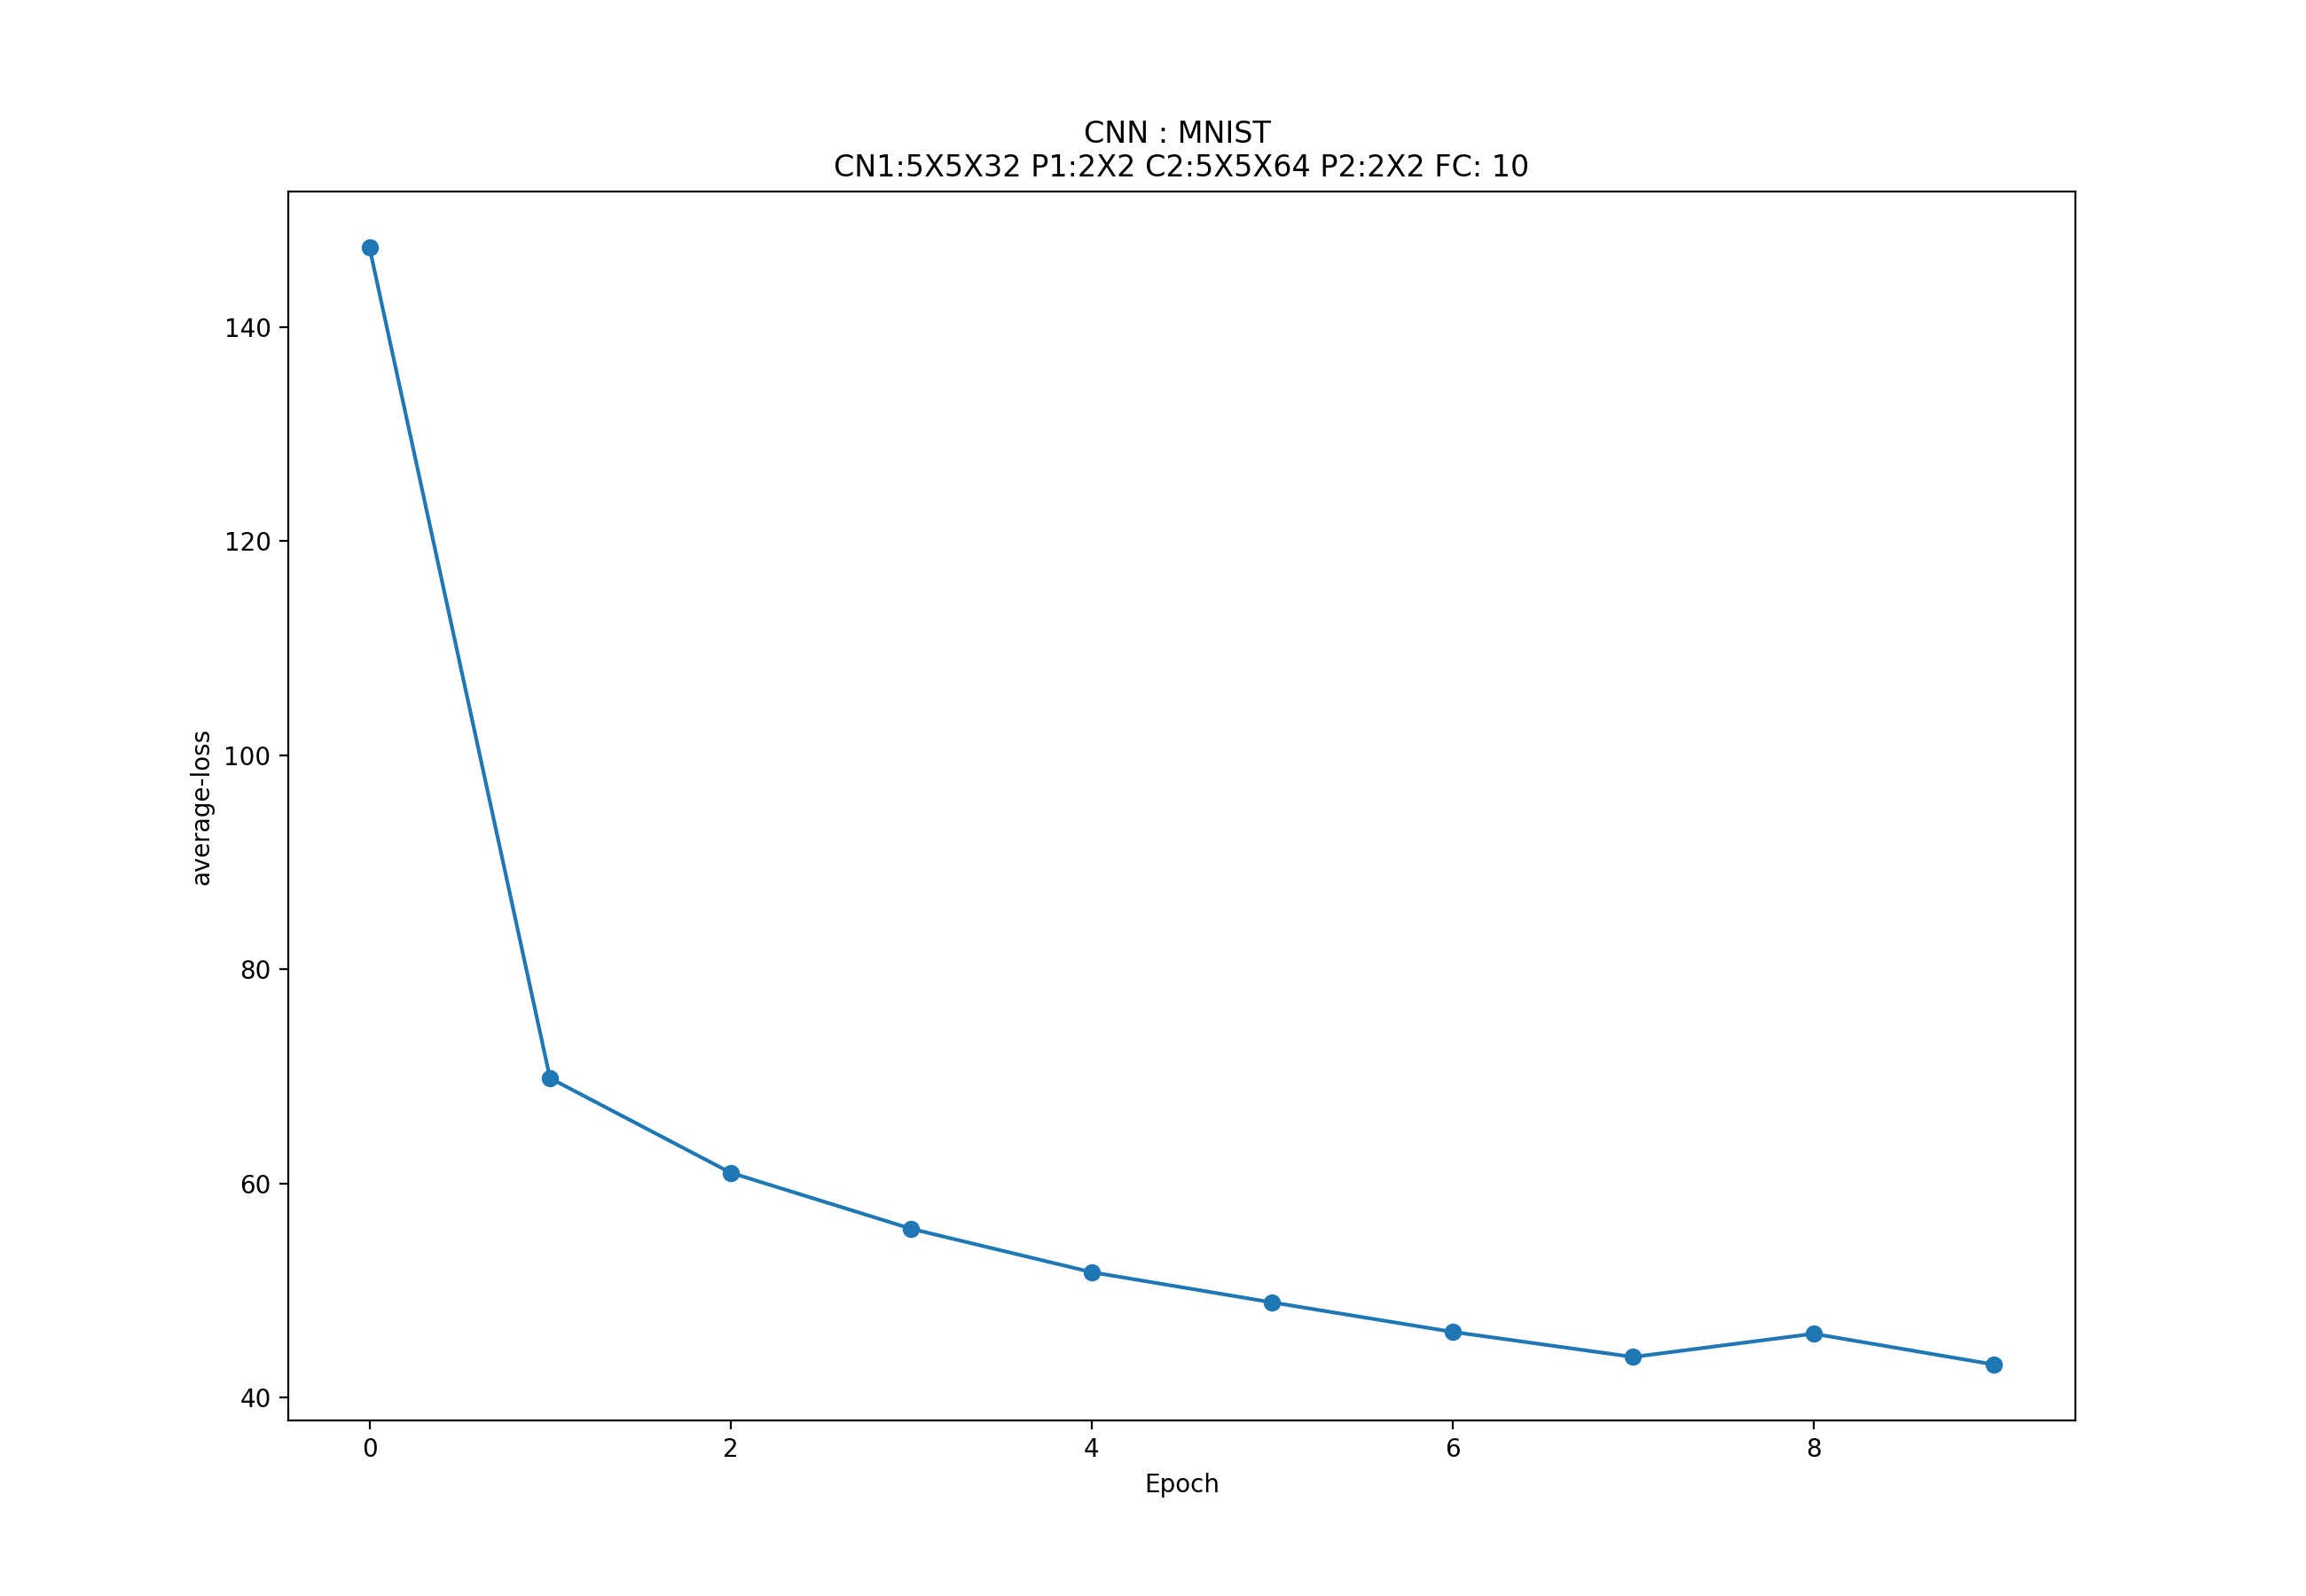
\includegraphics[width=0.5\linewidth]{MNIST-loss-decrease-CNNnotes-w-batch-100-lr-change.png}
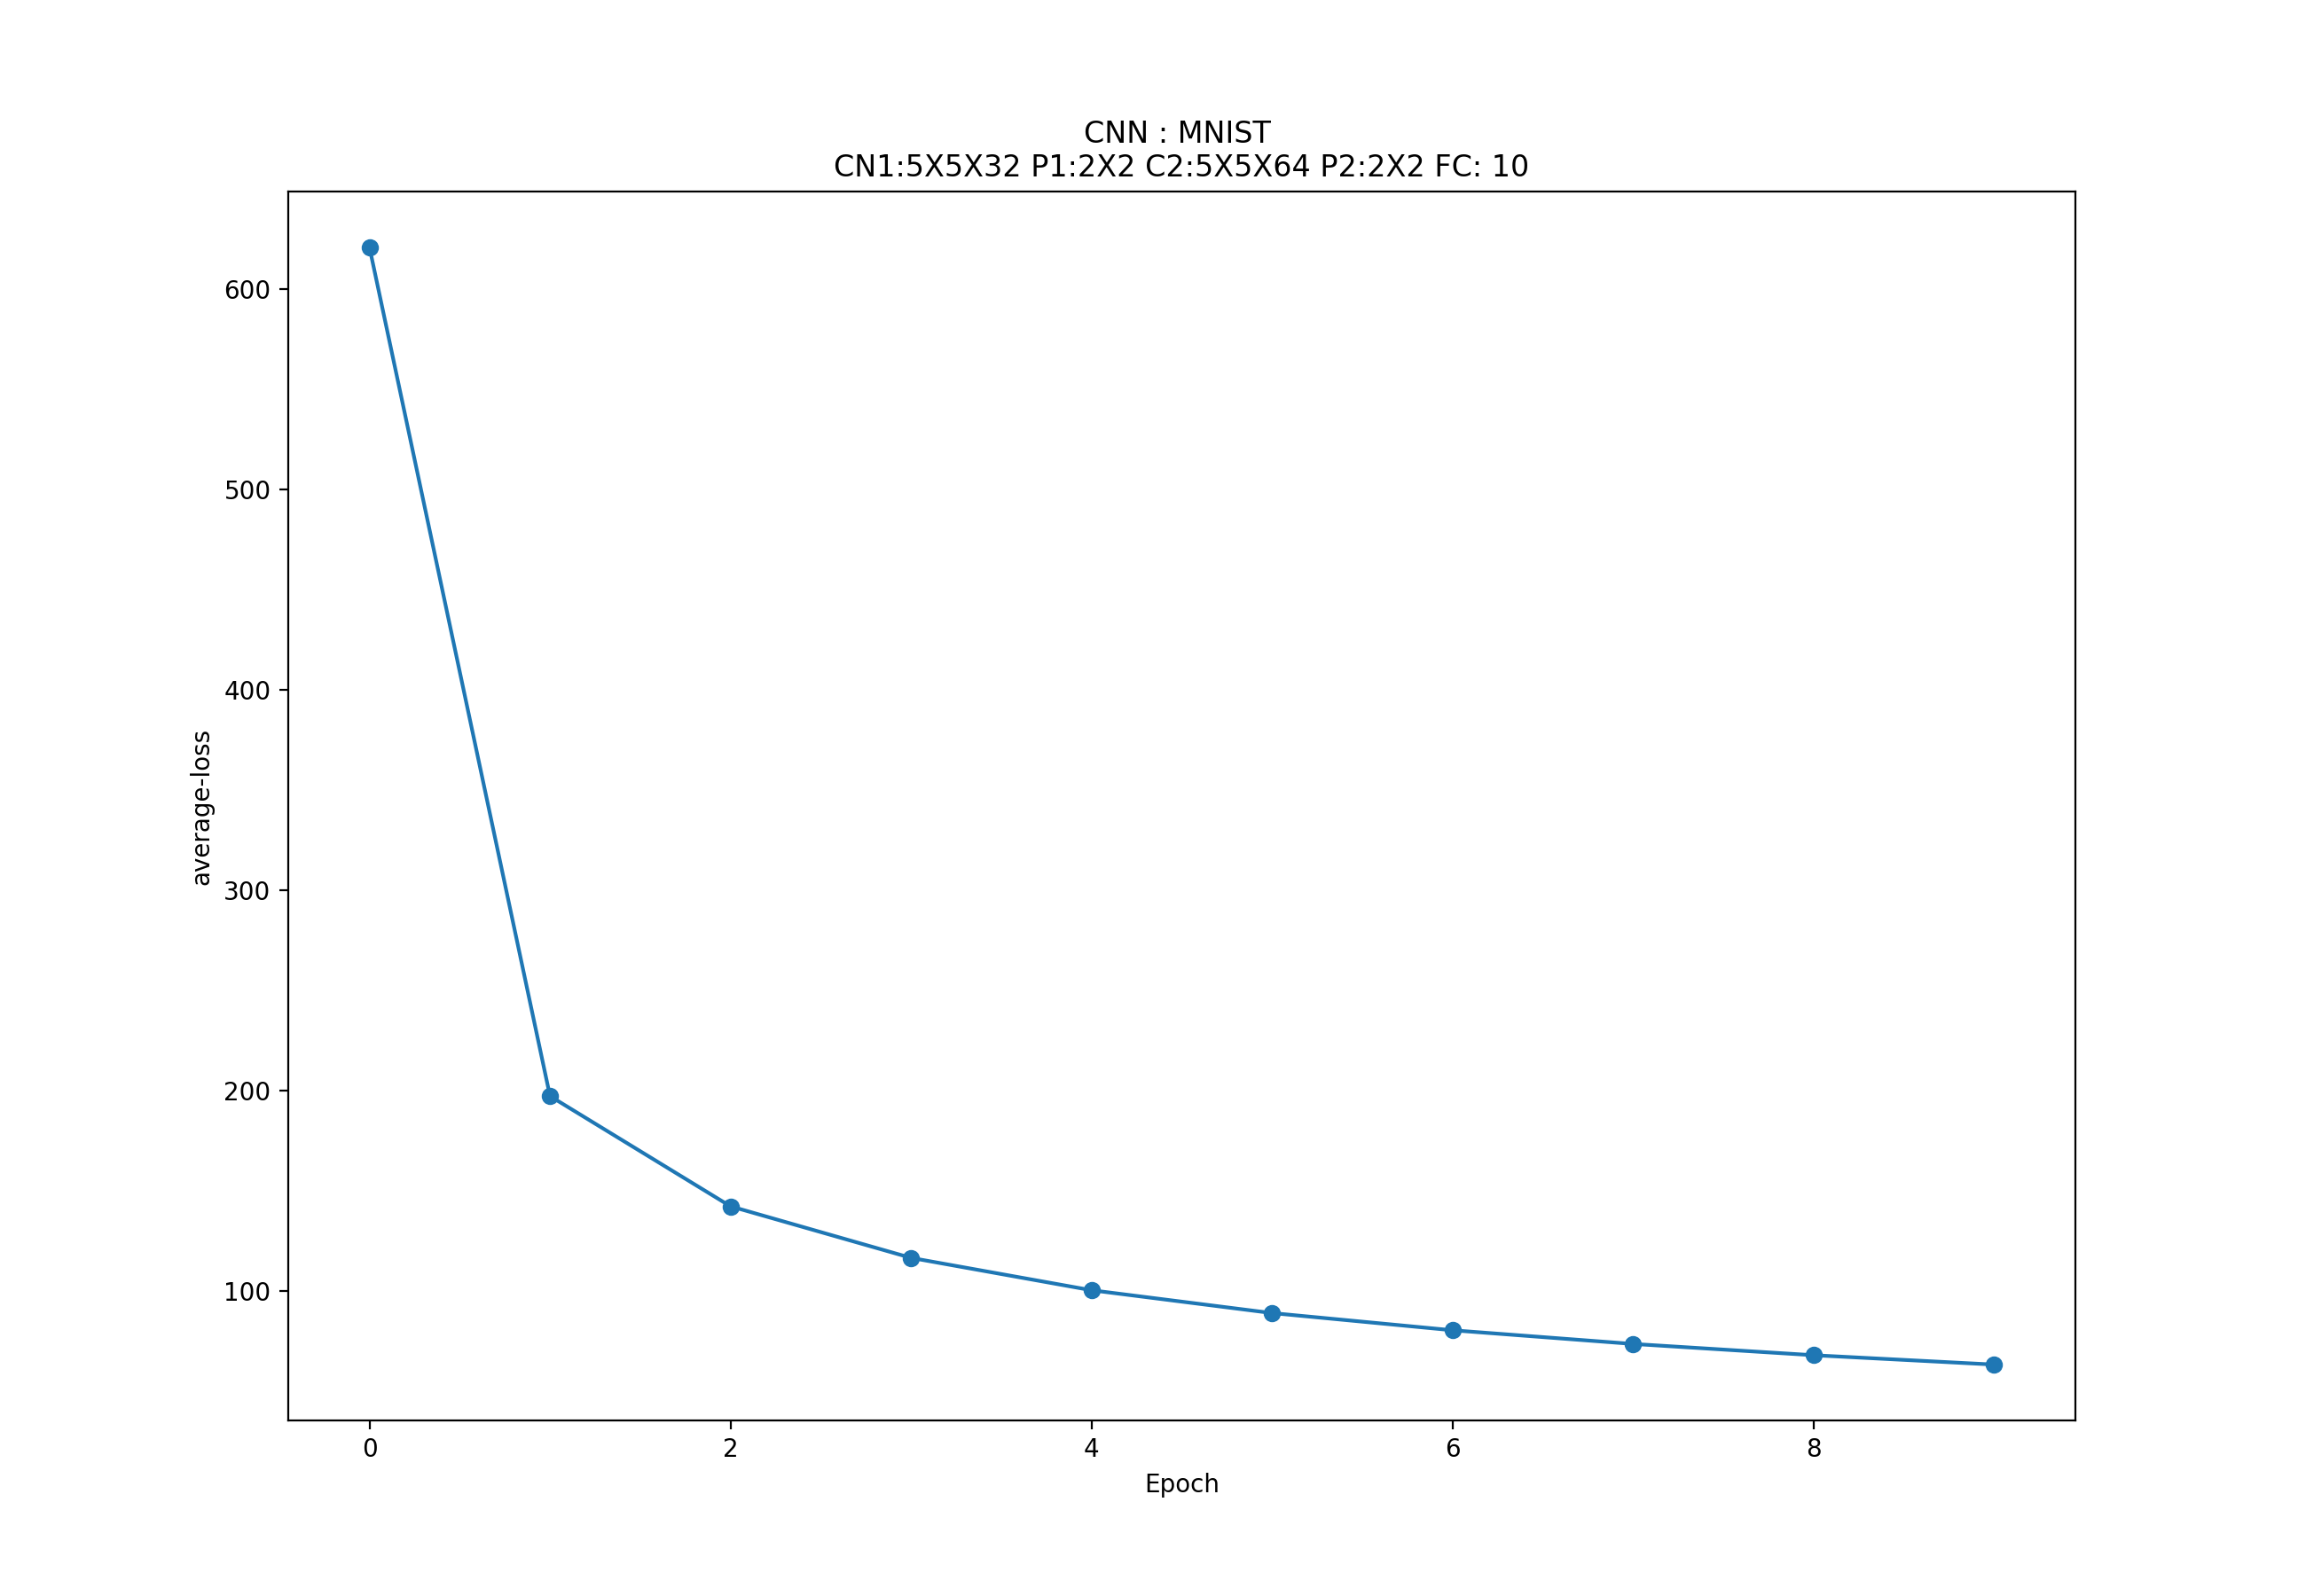
\includegraphics[width=0.5\linewidth]{MNIST-loss-decrease-CNNnotes-w-batch64.png}
\end{minipage}
\caption{Decrease in average loss with epoch on 4 different parameter configuration. Top Left : Config 1, Top Right: Config 2,
Bottom Left : Config 3, Bottom Right : Config 4}
\label{fig-3}
\end{figure}

Even though config 2, 3 and 4 show similar performance, it can be seen that they start at different loss values. With config-3 having the best starting point. It is however interesting to see that while config-4 starts at the worst point, it is slightly better than config-2 and config-3 on accuracy. Thus, learning rate, CNN specific parameters and batch size can all effect the performance of a CNN. 
\end{document}